\documentclass[a4paper, 14pt]{extarticle}
\usepackage[english, russian]{babel}
\usepackage[utf8x]{inputenc}
\usepackage{fullpage}
\usepackage{indentfirst} % Первый абзац в разделе тоже с красной строки
\usepackage{cmap} % для кодировки шрифтов в pdf (чтобы не было крокозябры при копировании из pdf )
\usepackage{graphicx} % для вставки картинок
\graphicspath{{res/}} % Путь к папке с картинками
\sloppy % Включение переноса слов в тексте

\title{Фреймворк для конечно-разностного моделирования диффузионных задач на гибридных вычислительных кластерах}
\author{Фролов Даниил Александрович}

% Для красивой вставки исходного программного кода 
\usepackage{listings}
\usepackage{color}

\definecolor{mygreen}{rgb}{0,0.6,0}
\definecolor{mygray}{rgb}{0.5,0.5,0.5}
\definecolor{mymauve}{rgb}{0.58,0,0.82}

% Параметры раскрски исходного кода программы 
\lstset{ %
	language = Java,
	extendedchars=\true, %Чтобы русские буквы в комментариях были
	%inputencoding=cp1251,
	%commentstyle=\itshape,
	%stringstyle=\bf,
  backgroundcolor=\color{white},   % choose the background color
  basicstyle=\footnotesize,        % size of fonts used for the code
  %basicstyle=\ttfamily\fontsize{11pt}{11pt}\selectfont,
  breaklines=true,                 % automatic line breaking only at whitespace
  captionpos=b,                    % sets the caption-position to bottom
  commentstyle=\color{mygreen},    % comment style
  escapeinside={\%*}{*)},          % if you want to add LaTeX within your code
  keywordstyle=\color{blue},       % keyword style
  stringstyle=\color{mymauve},     % string literal style
}

\usepackage{hyperref} % Для добавления ссылок в тесте

% Настройка цветов для ссылок
\hypersetup{
colorlinks = true,
linkcolor = black,
pagecolor = black,
urlcolor = blue, 
citecolor = black
}

% Математика
\usepackage{amssymb} % For use "mathbb" function
\usepackage{amsmath}
\usepackage{amsthm}
\usepackage{mathrsfs}
\newcommand{\La}{\mathscr{L}} % Функция Лагранжа
\newcommand{\ls}{{ℓ}} % Красивая l, чтобы легче было отличить от i, 1 b других палок
\providecommand{\norm}[1]{\lVert#1\rVert} % Норма вектора : ||w||
\newcommand{\dpt}[1]{\left\langle#1\right\rangle} % dot product using brackets
\newcommand{\brackets}[1]{\left(#1\right)} % Обернуть скобками автоматического размера
%\newcommand{\dpts}[2]{#2 \langle#1 #2 \rangle} % dot product using brackets with manual size
\newcommand{\R}{\mathbb{R}} % beautiful R for R^n labels
\newcommand{\il}{i = 1, \ldots, \ls} % writes i = 1, ..., l
\newcommand{\ili}{\quad i = 1, \ldots, \ls} % writes i = 1, ..., l with indent in begin
\newcommand{\sumil}{\sum_{i=1}^{\ls}} % Сумма по i, которая изменяется от 1 до l
\newcommand{\minl}{\min\limits} % min with limits under "min" label
\newcommand{\maxl}{\max\limits} % max with limits under "max" label

% Окружение для теорем, определений и т.д.
\theoremstyle{definition}
\newtheorem{definition}{Определение}
\newtheorem{theorem}{Теорема}
\newtheorem{example}{Пример}

% Поправить стиль отрисовки формул (особенно актуально для сумм https://ru.sharelatex.com/learn/Display_style_in_math_mode)
\everymath{\displaystyle}

%\bibliographystyle{unsrt} % упорядочить список использованной литературы по порядку упоминания их в тексте
\bibliographystyle{utf8gost705u}
%\bibliographystyle{utf8gost71u}

\usepackage[labelfont=bf, labelsep=space]{caption} % Делаем надписи "Рис.1" под рисунками жирными и без двоеточия.
\usepackage[top=20mm, bottom=20mm, left=30mm, right=20mm
, nohead % Убрать расстояние для верхних колонтикулов
%, nofoot % Убрать расстояние для нижних колонтикулов
]
{geometry} % Размер полей у старницы
\setlength{\parindent}{1.25cm} % Размер интервала для абзацев 
\usepackage{setspace}
\singlespacing % одинарный интервал
\renewcommand\normalsize{\fontsize{14}{16.8pt}\selectfont} % Сделать размер шрифта 14

\usepackage{caption} % подписи к рисункам в русской типографской традиции
\DeclareCaptionFormat{GOSTtable}{#2#1\\#3\vspace*{-\baselineskip}}
\DeclareCaptionLabelSeparator{fill}{\hfill}
\DeclareCaptionLabelFormat{fullparents}{\bothIfFirst{#1}{~}#2}
\captionsetup[table]{
     format=GOSTtable,
     %font={footnotesize},
     labelformat=fullparents,
     labelsep=fill,
     labelfont=normal,
     textfont=bf,
     justification=centering,
     singlelinecheck=false
     }

% Начинать каждую главу с новой страницы
\usepackage{titlesec}
\newcommand{\sectionbreak}{\clearpage}

% Позволяет подсчитывать число страниц в документе с помощью комманды \pageref*{LastPage}
\usepackage{lastpage}
%\pretolerance 10000

\begin{document}
\setcounter{tocdepth}{3}

% Позволяет подсчитывать число рисунков, таблиц и глав(section) в документе
\newcounter{totfigures}
\newcounter{tottables}
\newcounter{totsections}
\makeatletter
\AtEndDocument{%
	\addtocounter{totfigures}{\value{figure}}%
	\addtocounter{tottables}{\value{table}}%
	\addtocounter{totsections}{\value{section}}%
	\immediate\write\@mainaux{%
		\string\gdef\string\totfig{\number\value{totfigures}}%
		\string\gdef\string\tottab{\number\value{tottables}}%    
		\string\gdef\string\totsections{\number\value{totsections}}%  
	}%
}
\makeatother


%Титульный лист
{
\thispagestyle{empty}

\begin{center}
	
	Министерство образования и науки Российской Федерации\\[0.3cm]
	Государственное образовательное учреждение\\
	высшего профессионального образования\\
	"<Ярославский государственный университет им. П.Г. Демидова">\\
	(ЯрГУ)\\[0.3cm]
	
	Кафедра компьютерных сетей
	
	\bigskip
	
	\hspace{15em}"<Допустить к защите">
	
	\begin{flushright}
		Заведующий кафедрой\par
		д. ф.-м. н., профессор\par
		\underline{\hspace{3.2cm}}Глызин\,С.\,Д.\par
		"<\underline{\hspace{0.5cm}}">\underline{\hspace{3.4cm}}2015 г.\par
	\end{flushright}
	
	\bigskip
	
	{\textbf
		{\textit
			{Выпускная квалификационная работа бакалавра}
		}
	}
	\\
	по направлению 010400.62 Прикладная математика и информатика
	
	\bigskip
	
	{\bf
		Фреймворк для конечно-разностного моделирования диффузионных задач на гибридных вычислительных кластерах 
	}
\end{center}

\medskip

\begin{flushright}
	Научный руководитель\par
	д. ф.-м. н., профессор\par
	\underline{\hspace{3.5cm}}Глызин\,С.\,Д.\par
	"<\underline{\hspace{0.8cm}}">\underline{\hspace{3.5cm}}2015 г.\par
\end{flushright}

\bigskip 

\begin{flushright}
	Студент группы ИВТ-43-БО\par
	\underline{\hspace{2.5cm}}Фролов\,Д.\,А.\par
	"<\underline{\hspace{0.8cm}}">\underline{\hspace{3.5cm}}2015 г.\par
\end{flushright}

\vspace{\fill}

\begin{center}
	Ярославль 2015
\end{center}

\clearpage
}



%Реферат
\section*{Реферат}
\noindent Объем \pageref*{LastPage}~с., 
\totsections~гл., \totfig~рис., \tottab~табл., 
8 источников.
, ? прил. 

\noindent\textbf{Мои ключевые слова}

Мое описание

%Содержание
\tableofcontents





%Введение
\section*{Введение}
\addcontentsline{toc}{section}{Введение}

\par Развитие современного общества зачастую ставит перед наукой задачи, решение которых требует постороение моделей систем "<реакция-диффузия">.

\par Системы "<реакция-диффузия"> представляют собой важный класс нелинейных динамических систем, в которых пространственно неоднородные колебательные режимы обусловлены наличием диффузионной составляющей [1]. Такие системы часто встречаются в физических и биохимических приложениях, а также в задачах популяционной биологии [2].

\par В связи с вышесказанным проблема автоматизации моделирования диффузионных процессов является достаточно актуальной. Конечно, и ранее появлялись отдельные программные продукты, позволяющие моделировать тот или иной конкретный процесс, то есть решать вполне определенную, заранее заданную краевую задачу типа "<реакция-диффузия">.

\par Современный этап развития информатики и вычислительной техники позволяет подойти к решению этой задачи на более высоком уровне абстракции. Это означает, что можно создать программный комплекс, способный моделировать любою, заранее неизвестную, диффузионную задачу, конечно, при условии, что пользователь знает, какая математическая модель описывает этот процесс. Подобный комплекс позволит решать уже не одну конкретную, а множество задач из класса "<реакция-диффузия">. Этот программный комплекс должен обладать следующими качествами. Во-первых, высоким уровнем настраиваемости, то есть позволять пользователю задавать множество параметров: математическую модель, область задачи, точность вычислений, метод численного решения и другие. Во-вторых, программный комплекс должен работать эффективно, с высокой производительностью, в том числе на оборудовании с гибридной вычислительной системой и иерархической организацией памяти.

\par С учетом вышеизложенного перед автором работы была поставлена задача разработать часть программного комплекса, отвечающую за повышение его производительности. Решение этой задачи лежит в области распределенных вычислений, то есть применения современных методов распараллеливания с целью увеличения скорости работы.





%Первая глава
\section{Постановка задачи}

\subsection{Теоретические основы решения задач "<реакция-диффузия">}

\par Как известно, в общем случае уравнение "<реакция-диффузия"> представимо в виде краевой задачи:
$$\frac{\partial u}{\partial t} = D \frac{\partial^2 u}{\partial x^2} + F(u);$$
$$\left.{\frac{\partial u}{\partial x}} \right|_{x=0} = \left.{\frac{\partial u}{\partial x}} \right|_{x=1} = 0, F(0) = 0.$$

\par Для численного моделирования подобных задач возможно использовать подход, состоящий в приближении оператора Лапласа его разностными аналогами.
$$x_j = \bigtriangleup(j + \frac{1}{2}), \bigtriangleup = \frac{1}{N},$$
где N - количество отсчетов на оси.
$$\left.{\frac{\partial^2 u}{\partial x^2}}\right|_{x=x_j} = \frac{u_{j-1} - 2u_j + u_{j+1}}{\bigtriangleup^2};$$
$$\dot u_j = D\, \frac{u_{j-1} - 2u_j + u_{j+1}}{\bigtriangleup^2} + F(u_j);$$
$$u_0 = u_1, u_{N+1} = u_N, j = \overline{1, N}.$$

\par В результате подобных преобразований получается система обыкновенных дифференциальных уравнений. Для их численного решения применяются различные стандартные сеточные методы, в том числе метод Эйлера, метод Рунге-Кутты, Дормана-Принса.

\par Опишем стандартные методы численного решения начальной задачи Коши для систем обыкновенных дифференциальных уравнений. Метод Эйлера считается наиболее простым из подобных методов. Он относится к явным, одношаговым методам первого порядка точности и фактически основан на аппроксимации интегральной кривой кусочно-линейной функцией. Упрощенно метод Эйлера может быть представлен в следующем виде.

\par Пусть дана начальная задача Коши
$$\dot y = f(t, y)$$
и некоторое начальное условие
$$y(t_0) = y_0.$$

\par Тогда новое значение можно получить, с помощью предыдущего, используя следующее равенство:
$$y_{n+1} = y_n + \bigtriangleup t \cdot f(t, y_n).$$

\par Второй метод, который может быть использован для решения поставленной задачи, -- метод Рунге-Кутты. Данный метод кратко описывается следующей схемой.

\par Пусть дана такая же начальная задача Коши, что и для метода Эйлера. Тогда каждую последующую точку решения можно вычислить с помощью предыдущей, используя следующее равенство:
$$y_{n+1} = y_n + \sum_{i=1}^s b_i k_i.$$

\par Коэффициенты $k_i$ вычисляются, исходя из следующих соотношений:
$$k_1 = hf(t_n, y_n),$$
$$k_2 = hf(t_n + c_2 h, y_n + a_{21}k_1),$$
$$\cdots$$
$$k_s = hf(t_n + c_s, y_n + a_{s1}k_1 + a_{s2}k_2 + \cdots + a_{s,s-1}k_{s-1}).$$

\par Количество коэффицентов $k_i$ определяет порядок метода: к примеру, для четырехстадийной схемы Рунге-Кутты необходимо вычислить четрые таких коэффициента.

\par Для параметров $a_{ij}$, $b_i$, $c_i$, которые используются при расчеты $k_i$, должны выполняться следующие равенства:
$$\sum_{j=1}^{i-1}{a_{ij}} = c_i,$$
$$\sum_{j=1}^s{b_i} = 1,$$
$$0 \le (b_i, c_i, a_{ij}) \le 1,$$
$$b_i > 1.$$

\par Именно параметры $a_{ij}$, $b_i$ и $c_i$ задают конкретный метод Рунге-Кутты.

\par Как правило, для решения дифференциальных уравнений используются схемы невысоких порядков точности, поэтому в нашем случае достаточно воспользоваться четырехстадийной реализацией метода Рунге-Кутты, то есть взять $s = 4$.

\par Для решения задачи "<реакция-диффузия">, как уже было сказано выше, также может быть использован метод Дормана-Принса, который относится к классу методов Рунге-Кутты. По сравнению с последним он является более точным за счет большего числа стадий вычисления нового состояния. Среди особенностей метода также стоит отметить изменяемость шага вычислений.

\par Очевидно, что применение того или иного метода, оказывает влияние на точность и скорость производимых вычислений и, естественно, на конечный результат. В связи с этим, выбор конкретного метода решения следует оставить за пользователем.



\subsection{Основные требования к приложению}

\par Каждая конкретная задача "<реакция-диффузия">, которая может быть поставлена конечным пользователем, характеризуется несколькими параметрами. Во-первых, это краевая задача, описывающая происходящий физический, химический или биологический процесс. Во-вторых, для решения необходимо знать область, в которой этот процесс протекает. Назовем ее областью задачи. При этом необходимо учитывать, что область задачи может быть одномерной, двумерной или трехмерной и состоять из так называемых блоков. Для одномерного случая этими блоками являются отрезки, в случае плоскости - прямоугольники, а если область трехмерна - параллелепипеды. Каждый из блоков характеризуется координатами в пространстве и размерами, а также информацией о своих границах. Информация о границе блока содержит данные о поведении функции, которая моделирует процесс, в граничных точках. В качестве краевых условий могут использоваться условия Неймана или условия Дирихле. В первом случае задается поведение производной функции в граничных точках, а во втором - конкретные значения функции, заданные, возможно, с помощью другой функции. Следует заметить, что на разные участки границы могут быть наложены разные краевые условия. Область задачи может состоять из нескольких частей. Эти части, или блоки, могут иметь общую границу, точнее, место соединения. В этом случае на данный участок блоков не распространяются условия, заданные на границе, а место соединения считается внутренней областью.

\par На рисунке~\ref{ris:2Block_ex} представлен пример двумерной области, в которой моделируется уравнение теплопроводности. Указанная область состоит из двух прямоугольников, соединенных между собой. Место соединения обозначено пунктирной линией. Красным цветом выделена часть границы, на которой заданы условия Неймана с отрицательной производной, синим - условия Дирихле, зеленым - условия Неймана с положительной производной. На всей остальной границе области применяются условия Неймана с нулевой производной, что означает отсутствие теплообмена с внешней средой.

\begin{figure}[h]
	\center{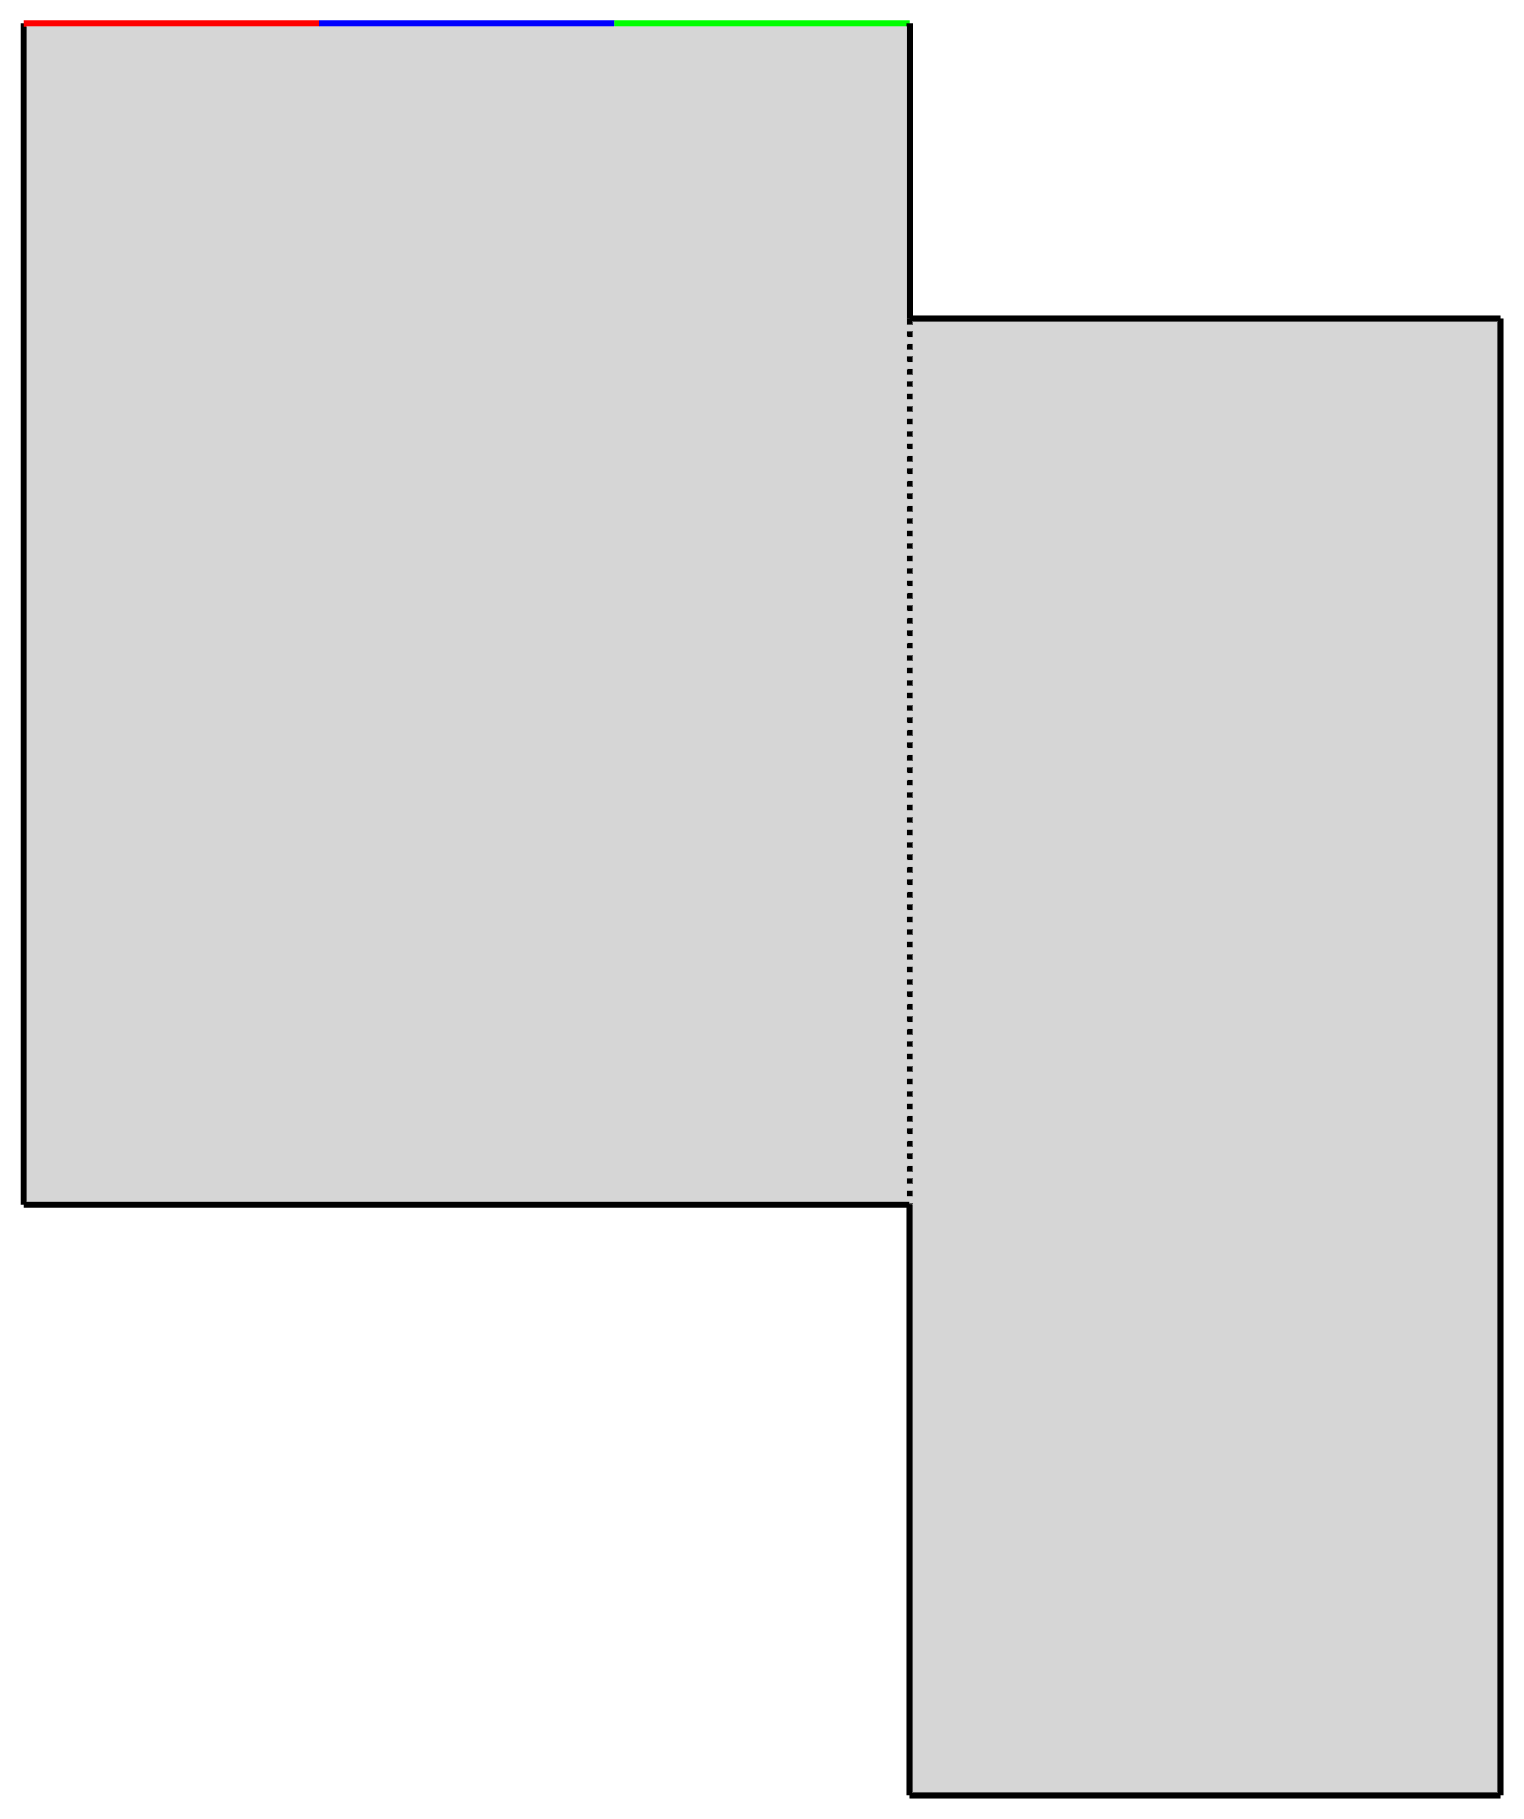
\includegraphics[width=0.7\linewidth]{2Block_ex.png}}
	\caption{Пример области задачи}
	\label{ris:2Block_ex}
\end{figure}

\par Последней составляющей, необходимой для начала работы приложения, является информация о начальном состоянии области задачи. Таким образом, для корректной работы приложения пользователь должен ввести следующие параметры:
\begin{enumerate}
\item[1)] моделируемая задача;
\item[2)] область задачи (координаты и размеры блоков);
\item[3)] граничные (краевые) условия;
\item[4)] места соединения блоков;
\item[5)] начальное состояние области задачи.
\end{enumerate}

\par Качественный современный программный продукт должен иметь возможность работы на оборудовании с гибридной вычислительной системой и иерархической организацией памяти. К гибридным системам относятся, например, вычислительные кластеры, которые используют для расчетов мощности центрального процессора и видеокарт. Иерархическая организация памяти предполагает малые объемы высокоскоростной памяти и большие - медленной. Подобный подход к реализации памяти подразумевает экономное расходование ресурсов в процессе выполнения с целью повышения общей производительности за счет ускоренного обращения к данным.

\par Ориентированный на пользователя программный продукт также должен обладать возможностью сохранять как окончательный, так и промежуточный результат вычислений и уметь и возобновлять работу с любого из сохраненных состояний. Кроме того необходимо обладать инструментами для запуска расчетов до определенного момента времени с данным шагом или выполнять заданное количество итераций.

\par В качестве языка программирования, используемого для реализации поставленных задач, был выбран C++ как наиболее подходящий для данных целей. Этот язык обладает необходимыми инструментами для удобной разработки подобного приложения, в частности, наличием механизма наследования. Кроме того язык C++ дает возможность низкоуровневой работы с памятью, что позволять эффективно осуществлять оптимизацию программного кода, направленную на повышение производительности.  Важным преимуществом С++ является наличие библиотеки MPI, с помощью которой производится передача данных между разными машинами, что очень важно при работе с вычислительными кластерами, имеющими в своем распоряжении несколько узлов, которые, в свою очередь, являются физически различными устройствами.




%Вторая глава
\section{Архитектура приложения}

\subsection{Класс Solver и его потомки}

\par Автоматизация моделирования задач "<реакция-диффузия">, как уже было сказано выше, требует использования численных методов решения. В данном проекте было реализовано несколько подобных методов:
\begin{enumerate}
\item[1)] метод Эйлера;
\item[2)] метод Рунге-Кутты;
\item[3)] метод Дормана-Принса.
\end{enumerate}

\par Первый методов является самым простым из всех перечисленных. Он включает в себя одну стадию вычислений и имеет постоянный шаг.

\par Метод Рунге-Кутты, представленный в проекте, аналогично первому методу имеет неизменяемый шаг, но использует четырехстадийную схему решения.

\par Последний метод использует семистадийную схему расчетов и отличается от двух ранее рассмотренных наличием изменяемого шага, а также необходимостью предварительной подготовки перед началом работы.

\par Для реализации всего вышеизложенного используются класс Solver и его наследники. Сам класс Solver лишь определяет интерфейс, которым должны обладать классы, реализующие методы численного решения.

\par В процессе работы необходимо знать некоторую общую информацию об используемом методе, для того чтобы корректно продолжать вычисления. Например, нужно знать сколько стадий необходимо методу и нужно ли выполнять изменение шага по времени. Подобную информацию содержат классы EulerSolver, RK4Solver и DP45Solver, которые являются наследниками Solver'а. Каждый из них обладает всей информацией о методе, которая может потребоваться в процессе вычислений: количество стадий, тип шага (постоянный или изменяемый), необходимость предварительной подготовки. Кроме того здесь же содержатся различные константы, необходимые методу. Например, в DP45Solver это могут быть минимальный и максимальный коэффициенты изменения шага. Все эти классы не хранят данные о текущем состоянии решения, они предназначены исключительно для предоставления справочной информации.

\par Полноценными классами, способными хранить данные, являются наследники вышеописанных классов, а именно EulerSolverCpu, EulerSolverGpu, RK4SolverCpu, RK4SolverGpu и так далее. Как видно из названий этих классов, каждая пара предназначена для работы на центральном процессоре и видеокарте соответственно. Подобное решение продиктовано разным способами выделения памяти и работы с ней на двух этих типах устройств.

\par Общую схему классов можно увидеть на рисунке~\ref{ris:solvers}.

\begin{figure}[h]
	\center{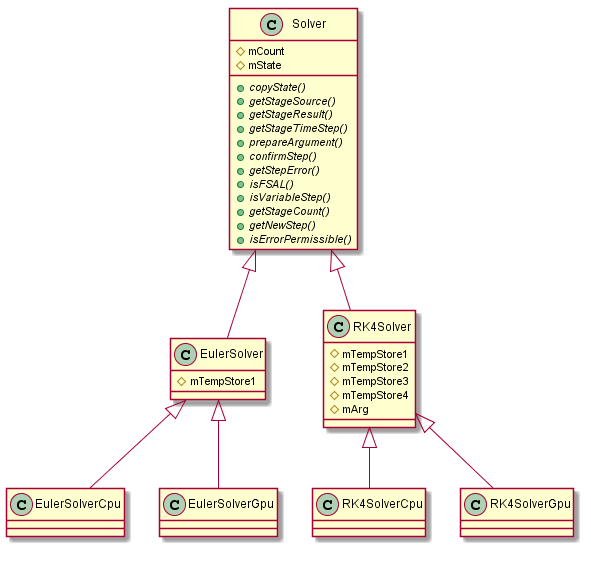
\includegraphics[width=1.0\linewidth]{solvers.png}}
	\caption{Иерархия наследования для методов численного решения}
	\label{ris:solvers}
\end{figure}

\par Рассмотрим подробнее работу данных классов на примере RK4SolverCpu. Экземпляр данного класса фактически является "<хранилищем"> данных. Текущее состояние хранится в mState, данное поле имеют все без исключения классы, реализующие различные численные методы. Кроме того существует несколько дополнительных "<хранилищ"> (mTempStore1, mTempStore2, mTempStore3, mTempStore4), они используются для сохранения результатов вычисления на разных стадиях. Последний подобный "<склад">  это mArg, он необходим при получении нового состояния с использованием результатов, полученных ранее при выполнении четырех стадий метода.

\par В процессе вычислений объект данного класса выдает источник данных и их приемник, для этого используются описанные ранее переменные. Например, на первой стадии в качестве источника информации будет предоставлено mState, а запишется информация в mTempStore1. Стоит отметить, что сам объект не занимается непосредственно вычислениями, это работа другого класса. После каждой стадии метода выполняется функция prepareArgument(), она занимается необходимой обработкой полученных данных перед следующей итерацией метода.

\par После того, как шаг метода выполнен, выполняется его подтверждение (confirmStep()) или он отвергается. Данное действие необходимо, так как некоторые методы, например, метод Дормана-Принса, могут не принимать результаты, если сочтут погрешность вычислений слишком большой. При этом будет предпринята попытка получить новое состояние с меньшим шагом. Надо отметить, что метод Рунге-Кутты является методом с постоянным шагом и никогда не отвергает полученные результаты, поэтому функция подтверждения шага для этого метода просто меняет местами содержимое mState и mArg, так как в последнем будет храниться новое состояние.



\subsection{Класс Block и его потомки}

\par Обсуждая вопрос архитектуры системы, невозможно обойти одну из самых важных составляющих приложения - блоки. Область, над которой производятся вычисления, разбивается на составные части, называемые блоками. Для их представления используются класс Block и его потомки.

\par Класс Block является абстрактным классом и необходим для описания свойств, которые присущи всем блокам независимо от того, на каком типе устройства они будут выполняться. Например, к таким свойствам можно отнести размерность. Каждый блок может быть одномерным, двумерным или трехмерным в зависимости от поставленной задачи. Кроме того каждый блок обладает определенными координатами в пространстве и размерами. Важной информацией о блоке также является тип устройства, на котором будет производится вычисление конкретно данного блока, и номер устройства. Хранение этих данных тоже предусмотрено в указанном классе.

\par Каждый блок должен обладать определенным набором методов, которые описаны в классе Block. К таким методам относятся, например, вычисление нового состояния (computeStageCenter() и computeStageBorder()), подготовка к новой стадии численного метода (prepareArgument()), подтверждение выполненного шага и другие. Все эти методы позволяют полноценно работать с блоком и осуществлять вычисления.

\par Всего у класса Block существует три наследника (см. Рис.~\ref{ris:blocks}):
\begin{enumerate}
\item[1)] BlockCpu;
\item[2)] BlockGpu;
\item[3)] BlockNull.
\end{enumerate}

\begin{figure}[h]
	\center{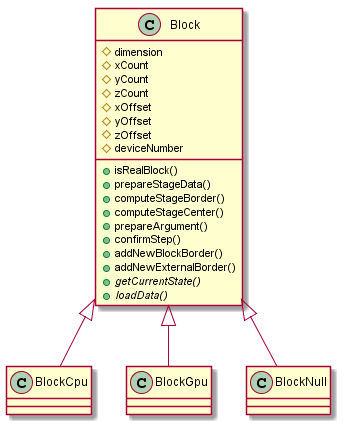
\includegraphics[width=0.7\linewidth]{blocks.png}}
	\caption{Иерархия наследования для блоков}
	\label{ris:blocks}
\end{figure}

\par Первые два класса-наследника работают на центральном процессоре и видеокарте соответственно. Как и в случае с Solver'ами подобное разделение обусловлено различными способами работы с памятью, но в данном случае это не единственная причина. В зависимости от типа устройства меняется и способ осуществления параллельных вычислений: для центрального процессора используется библиотека OpenMP, а для видеокарты -- язык CUDA. Подробнее это будет рассмотрено в одной из следующих глав. Объекты этих классов создают себе "<хранилища"> (наследников класса Solver) для работы с данными и реально занимаются вычислениями.

\par BlockNull -- класс-наследник Block, который никаким образом не хранит данные о текущем состоянии той части области, за которую он формально отвечает. Он нужен для того, чтобы обозначить, что составляющая области, относящаяся к данному блоку, на самом деле обрабатывается другим потоком и на другой машине. Но он позволяет выполнить все функции, присущие блоку: получение координат и размеров, даже выполнение расчетов, правда, в данном случае ничего рассчитано не будет.

\par Отдельно стоит осветить вопрос пользовательских функций. Задача реализации высокого уровня абстракции предполагает генерацию программного кода по пользовательским функциям. Наряду с областью, над которой выполняются вычисления, пользователь задает систему уравнений, которую необходимо моделировать, граничные условия и начальное состояние. Исходя из полученных данных формируется набор пользовательских функций, которые необходимы для работы приложения. В этот набор входят функции, которые задают начальное состояние области, а также функции, позволяющие рассчитать новое значение в определенной ячейке блока.

\par Поскольку обработка области задачи может происходить только дискретно, каждый блок разбивается на ячейки, количество которых зависит от указанной пользователем степени разбиения. В связи с этим каждый блок имеет специальную матрицу, которая совпадает по размеру с количеством ячеек, относящихся к блоку. Очевидно, что алгоритм расчета нового состояния для граничных ячеек может отличаться от алгоритма, который используется для внутренних ячеек. Это обусловлено тем, что обычно новое состояние каждой ячейки зависит от текущего состояния ее соседей, а у граничных ячеек набор соседей неполный. В матрице блока хранятся индексы функций, которые ответственны за перерасчет конкретно данной ячейки. На этапе подготовки выполняет компиляция пользовательских функций и формирование списка указателей на них. Индексы из этого списка и заносятся в матрицу. Функция для любой ячейки имеет унифицированную сигнатуру, что позволяет удобным образом осуществлять ее вызов, не задумываясь об особом статусе ячейки, если таковой имеет место быть.



\subsection{Класс Interconnect}

\par В процессе вычислений блокам требуется информация, которую необходимо получить от других составляющих области. Поэтому в контексте рассмотрения класса для передачи информации между блоками полезно заострить внимание на особенностях, связанных с их размещением. Очевидно, что существует три варианта размещения каждой пары блоков друг относительно друга:
\begin{enumerate}
\item[1)] блоки располагаются на одном вычислительном устройстве;
\item[2)] блоки размещаются на разных устройствах в пределах одной машины;
\item[3)] блоки находятся на разных машинах.
\end{enumerate}

\begin{figure}[h]
	\begin{minipage}[h]{0.3\linewidth}
		\center{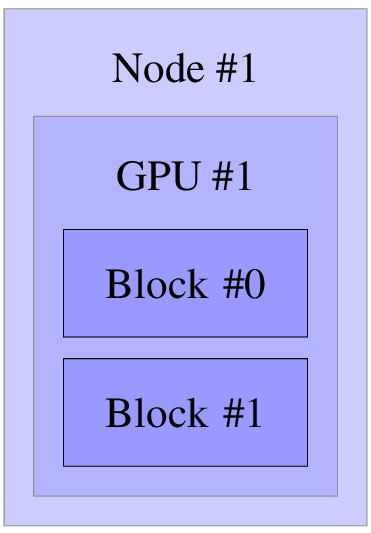
\includegraphics[width=0.7\linewidth]{1Node_1Device_2Block.png} \\ Одно устройство}
	\end{minipage}
	\hfill
	\begin{minipage}[h]{0.6\linewidth}
		\center{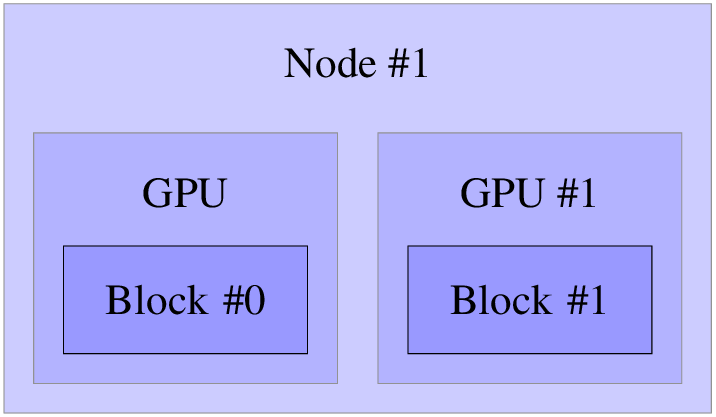
\includegraphics[width=0.85\linewidth]{1Node_2Device_2Block.png} \\ Два устройства на одной машине}
	\end{minipage}
	\hfill
	\begin{minipage}[h]{1.0\linewidth}
		\center{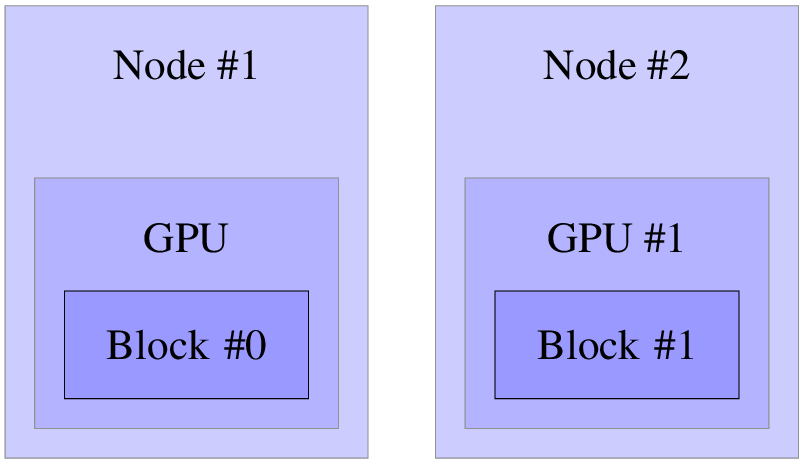
\includegraphics[width=0.6\linewidth]{2Node_2Device_2Block.png} \\ Два устройства на разных машинах \\ ~ }
	\end{minipage}
	\caption{Варианты расположения блоков}
	\label{ris:var}
\end{figure}

\par В случае расположения блоков на одном вычислительном устройстве проблема обеспечения доступа одного блока к данным, складируемым другим, фактически отсутствует, так как в данной ситуации нет ограничения для доступа к памяти.

\par Во втором случае существуют ограничения, вызванные тем, что центральный процессор не имеет возможности напрямую читать из памяти видеокарты, также как и видеокарта не может осуществлять подобные манипуляции с памятью центрального процессора. Эти же ограничения возникают и в случае расположения блоков на двух разных видеокартах. Данная проблема решается путем выделения памяти под данные, которые необходимы другим блокам, в специальной области, доступ к которой имеют оба вида вычислительных устройств. Этот вид памяти обычно называют pinned-память.

\par Основные трудности связаны с передачей информации в третьем случае. Расположения блоков на разных машинах делает невозможным прямое обращение к памяти и получение информации. Для решения данной проблемы и создан класс Interconnect. Объекты данного класса используются для пересылки данных между блоками, которые располагаются на различных узлах вычислительного кластера. Каждый экземпляр класса хранит номер потока, являющегося источником информации, то есть потока, к которому реально приписан интересующий нас блок (для удобства будем называть его Потоком №1). Кроме того в нем содержится номер потока, который является приемником информации (Поток №2). Заметим, что поток - приемник информации обслуживает некий другой блок, связь с которым необходимо реализовать. Для организации процесса передачи данных каждый объект класса Interconnect содержит два указателя на область памяти: первый - на массив данных, сформированный блоком-источником и расположенный в зоне ответственности Потока №1, второй - на массив данных, откуда впоследствии блок-приемник сможет получить интересующую его информацию в части обработки соединения между двумя этими конкретными блоками. Очевидно, что второй массив располагается в области памяти Потока №2. Кроме вышеперечисленных полей объект класса Interconnect содержит длину массива передаваемой информации.

\par Таким образом, структуру экземпляра класса Interconnect можно представить в следующем виде:
\begin{enumerate}
\item[1)] номер потока-источника;
\item[2)] номер потока-приемника;
\item[3)] указатель на область памяти, содержащей данные, которые необходимо переслать;
\item[4)] указатель на область памяти, предназначенной для приема передаваемых данных;
\item[5)] длина массива передаваемой информации.
\end{enumerate}

\par Все указанные данные необходимы для корректной работы библиотеки MPI, которая используется для передачи данных.

\par Каждый поток исполнения создает экземпляр класса Interconnect для обслуживания связи между парой блоков. Подобные объекты создаются на любую связь между блоками, даже если ни один из блоков данного соединения не относится к рассматриваемому потоку. В качестве пояснения приведем следующий пример. Пусть область задачи состоит из трех блоков: №0, №1 и №2, распределенных на трех разных потоках. Предположим, что блок №1 соединен с блоком №0 и блоком №2 (см. Рис.~\ref{ris:3Block_ex}). В этом случае для каждого потока будет создано четыре объекта класса Interconnect, обслуживающие следующие связи:
\begin{enumerate}
\item[1)] {№0 $\to$ №1};
\item[2)] {№1 $\to$ №0};
\item[3)] {№1 $\to$ №2};
\item[4)] {№2 $\to$ №1}.
\end{enumerate}

\begin{figure}[h]
	\center{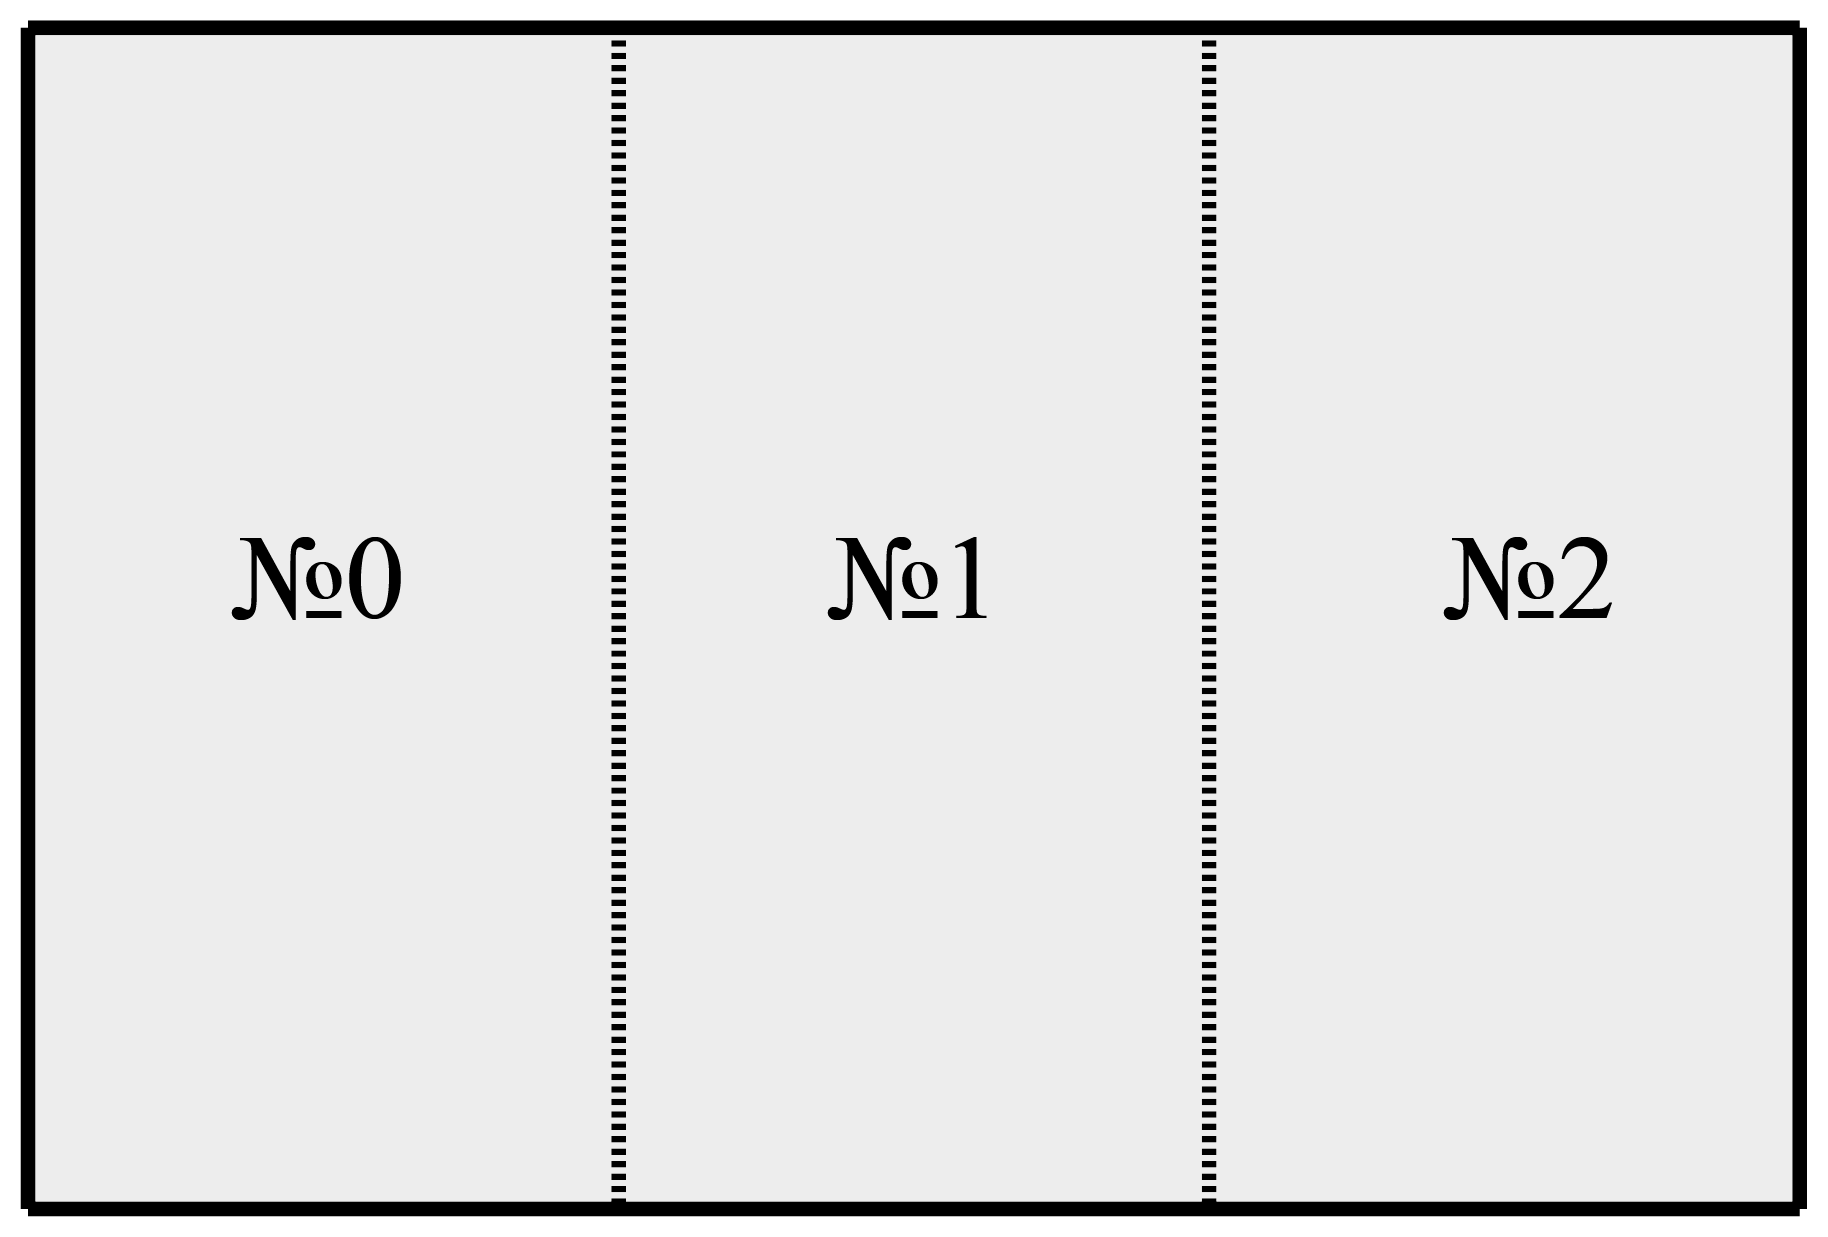
\includegraphics[width=0.8\linewidth]{3Block_ex.png}}
	\caption{Пример трех блоков}
	\label{ris:3Block_ex}
\end{figure}

\par Стоит обратить внимание, что блок №0 не имеет никакой связи с блоком №2, но при этом обслуживающий его поток создаст все четыре объекта, в том числе {№1 $\to$ №2} и {№2 $\to$ №1}. 

\par При вызове функции передачи~/~приема экземпляр класса выполняет одно из следующих действий:
\begin{enumerate}
\item[1)] выход без передачи данных;
\item[2)] отправка сообщения с данными;
\item[3)] прием сообщения с данными.
\end{enumerate}

\par Выход без передачи данных возникает, во-первых, если номер потока-отправителя совпадает с номером потока-получателя, что означает, что блоки располагаются в пределах одной машины, а, возможно, даже на одном устройстве. Понятно, что в подобной ситуации пересылка как таковая не требуется. Второй случай выхода без передачи возможен, если вызвавший поток не имеет отношения к обрабатываемой связи. В приведенном примере он произойдет, когда поток, обслуживающий блок №0, вызовет функцию передачи~/~приема на экземпляре класса Interconnect {№1$\to$ №2} или {№2 $\to$ №1}.



\subsection{Класс Domain}

\par Главным управляющим классом приложения является класс Domain. Объект данного класса создается в единственном экземпляре каждым потоком. Предполагается, что на одном вычислительном узле не запускается более одного потока. Подобное ограничение введено с целью исключить следующую ситуацию. Предположим, на одной машине одновременно выполняются два или более потоков. Каждый из них имеет некоторое количество блоков, и вполне вероятно, что некоторые блоки, принадлежащие разным потокам, окажутся на одном вычислительном устройстве. Кроме того очевидно, что все блоки располагаются в пределах одной машины. Как было описано ранее, в подобной ситуации передача данных между блоками средствами библиотеки MPI не требуется, так как ее можно организовать проще и, что еще более важно, она может осуществляться быстрее. Но в случае, который сейчас рассматривается, передача информации будет осуществляться именно через стороннюю библиотеку. Иллюстрация неоптимизированной передачи данных в этом случае приведена на рисунке~\ref{ris:error_ex}. С целью предотвращения подобной ситуации и было введено данное ограничение, которое фактически не мешает полноценному функционированию приложения.
\begin{figure}[h]
	\center{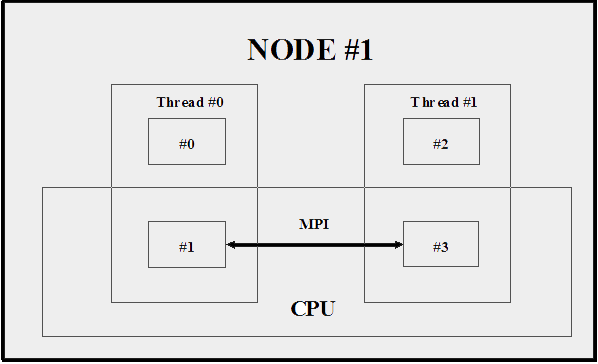
\includegraphics[width=0.8\linewidth]{error_ex.png}}
	\caption{Иллюстрация неоптимизированной передачи данных}
	\label{ris:error_ex}
\end{figure}

\par Объекты класса Domain осуществляют управление вычислениями каждый на своем потоке. В начале выполнения считывается файл, содержащий всю необходимую информацию о решаемой задаче: количество блоков, их размерность, размеры и координаты, а также данные о связях между блоками и другие сведения. Все это позволяет полностью сформировать набор переменных для дальнейшего решения (см. Рис.~\ref{ris:all}). Основную часть этих переменных, конечно, составляют блоки и связи между ними. Кроме того здесь же выполняется присвоение значений таким переменным, как номер потока выполнения, количество потоков в целом, количество блоков и соединений. Также создается объект класса-наследника Solver, который будет предоставлять необходимую информацию о численном методе, применяющемся для решения задачи.
\begin{figure}[h]
	\center{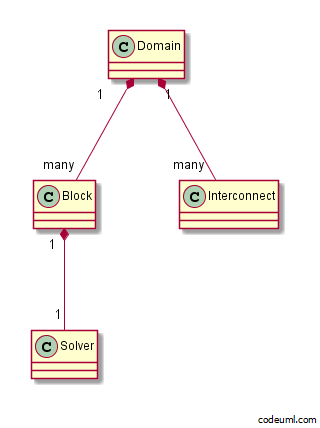
\includegraphics[width=0.55\linewidth]{all.png}}
	\caption{Схема классов}
	\label{ris:all}
\end{figure}



\subsection{Схема работы приложения}

\par Прежде чем переходить к рассмотрению схемы работы приложения (см. Рис.~\ref{ris:scheme}) необходимо ввести понятия центральных и граничных элементов блока.

\begin{figure}[h]
	\center{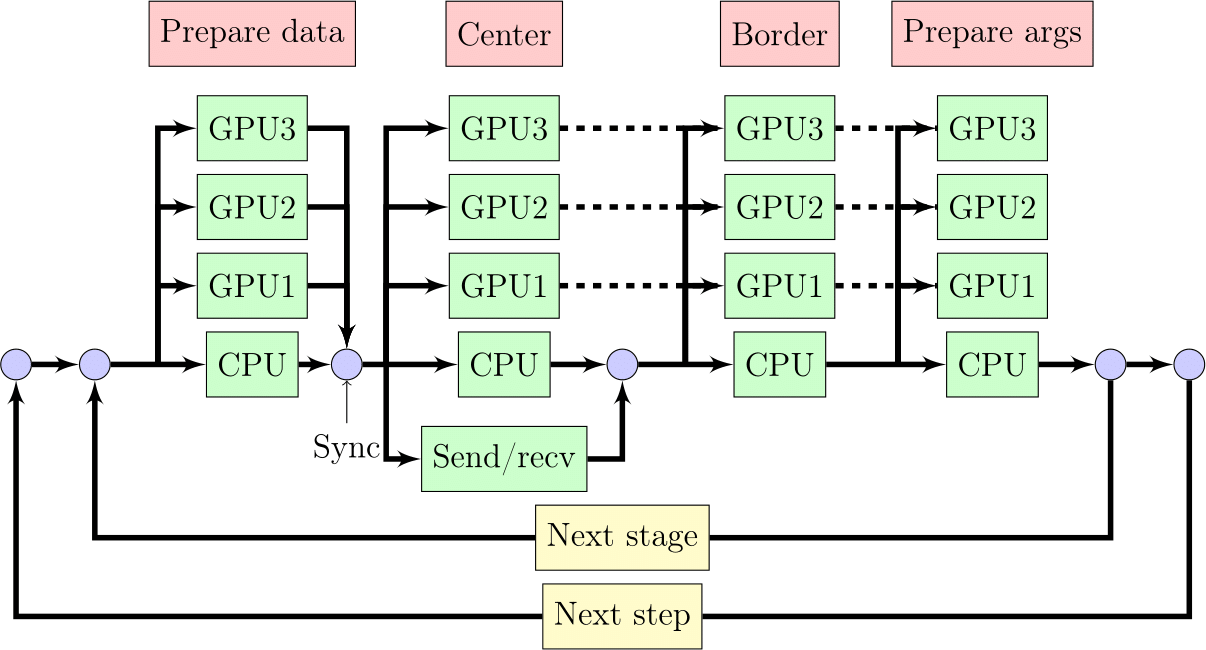
\includegraphics[width=1.0\linewidth]{scheme.png}}
	\caption{Схема вычислений}
	\label{ris:scheme}
\end{figure}

\par Центральными элементами будем называть такие элементы, для вычисления новых значений которых не требуются данные от других блоков.

\par Граничные элементы - это элементы, для вычисления новых значений которых могут потребоваться данные от других блоков, следовательно, не исключена возможность пересылки данных между различными вычислительными узлами кластера.

\par После того, как выполнена полная инициализация задачи, можно начинать вычисления. На каждом потоке объект управляющего класса вызывает функцию compute(), которая начинает вычисления. До тех пор, пока не выполнено необходимое условие, будут выполнять действия, представленные на рисунке~\ref{ris:scheme}. Сначала каждый блок выполняет подготовку данных, то есть копирует часть своей информации, необходимой его  "<соседям"> - блокам, с которыми у него есть связь. Подобные действия выполняет каждый блок на каждой машине.

\par Важным опорным элементом алгоритма является точка синхронизации. В этом момент времени можно быть уверенным, что все потоки пришли в эту точку и дождались друг друга. Это необходимо для того, чтобы потоки не обгоняли друг друга. Например, область состоит из двух блоков, но один из них оказался значительно больше другого. В такой ситуации поток, работающий с блоком меньшего размера, будет выполнять вычисления значительно быстрее и предоставлять некорректные данные для пересылки. Решение в конечном итоге окажется неверным. Для исключения подобной ситуации введена синхронизация потоков. Важно отметить, что инициализация новых вычислений или подготовка данных на центральном процессоре невозможны до завершения предыдущих действий, а каждый вызов вычислений с помощью ядра видеокарты всегда дожидается завершения предыдущего вызова на этой видеокарте.

\par После завершения этих действий имеются полностью подготовленные массивы, которые и будут пересылаться между вычислительным узлами кластера. Если пересылка не требуется, то блоки будут брать информацию именно из этих массивов напрямую, иначе инициализируется процесс пересылки данных. Этот процесс требует значительных временных затрат, которые вполне разумно использовать для вычисления той части блоков, которым пересылаемые данные не могут потребоваться в принципе, то есть для вычисления новых значений центральных элементов. В связи с этим передача данных выполняется асинхронным образом, то есть после вызова команды "<отправить"> процесс, вызвавший ее, не дожидается завершения операции, а продолжает работу. Аналогичным образом поступает и поток, который информацию будет принимать. Он просто сигнализирует о том, что готов это сделать, но не дожидается окончания передачи данных. Пока информация пересылается, ведется расчет центральных элементов. Вычисления запускаются одновременно на центральном процессоре и видеокартах. Каждое устройство будет выполнять вычисления только с блоками, которые принадлежат этому устройству. Если окажется, что таких блоков нет, то устройство просто завершит выполнения данной части алгоритма.

\par После того, как процессор завершил расчет центральных элементов, относящихся к его блокам, он запускает ожидание окончания пересылки. Так как передача данных выполнялась асинхронным образом, обязательно нужно убедиться, что действие завершено прежде чем приступать к пересчету граничных элементов, новые значения которых могут зависеть от этих данных. Указанные вычисления осуществляются аналогично вычислениям центральных элементов.

\par Далее необходимо выполнить подготовку аргументов, так как при использовании многостадийного метода может потребоваться, например, сумма матриц, полученных на предыдущих стадиях, а это дополнительные вычисления, которые можно и нужно распараллелить. Затем  производится переход или на следующую стадию метода, или к следующей итерации - выполнение шага по времени. Данный процесс длится до тех пор, пока не будут достигнуты заданные условия или пользователь не остановит процесс принудительно.





%Третья глава
\section{Компоненты программного комплекса}

\subsection{Общие сведения}

\par Важной составляющей программного комплекса, ориентированного на конечного пользователя является пользовательский интерфейс. В его задачи входит предоставление удобных инструментов для управления задачами и вычислениями, а именно: создание и сохранение проектов, запуск, приостановка и завершение вычислений, визуализация полученных результатов.

\par Значимую роль в работе приложения играет программа предварительной обработки. Данная часть комплекса ответственна за преобразование пользовательских функций в код, который впоследствии будет скомпилирован и использован при расчетах. Кроме того данная часть приложения разбивает область задачи на блоки и осуществляет их распределение по вычислительным устройствам и узлам кластера, а также создает бинарный файл со всей необходимой информацией, который передается вычислительному ядру для дальнейшей работы и вычислений на его основе.

\par Наконец, параллельный фреймворк, или вычислительное ядро, занимается непосредственно распределенными вычислениями. Задачей этой части программного комплекса является непосредственное осуществление параллельного выполнения расчетов на вычислительном кластере.



\subsection{Параллельный фреймворк}

\par Поговорим чуть подробнее о механизмах и инструментах, которые используются при распределенных вычислениях. Фактически распараллеливание проводится в два этапа:
\begin{enumerate}
\item[1)] разделение задачи на блоки - крупнозернистый параллелизм;
\item[2)] параллельные вычисление на устройстве - мелкозернистый параллелизм.
\end{enumerate}

\subsubsection{Крупнозернистый параллелизм}

\par Крупнозернистый параллелизм осуществляется путем разбиения области на блоки и распределения блоков по вычислительным устройствам еще на этапе подготовки, о чем было рассказано в предыдущих главах. Данный подход позволяет использовать все вычислительные мощности, имеющиеся в наличии, и равномерно распределять нагрузку на устройства. На одном устройстве может располагаться несколько блоков одновременно, в таком случае их вычисление будет осуществляться в порядке очереди. Немаловажным фактом является то, что в случае, если количество блоков значительно (в несколько раз) превышает количество вычислительных устройств, то блоки, которые имеют общие границы, разумно располагать на одном устройстве, либо в пределах одной машины, а блоки, не имеющие таких границ, -- на разных, сохраняя равномерность распределения блоков по устройствам в целом. Такой подход позволяет увеличить скорость расчетов для небольших по количеству используемых ячеек областей. Достигается это уменьшением времени, которое необходимо на пересылку данных от одного блока к другому между итерациями вычислений. Очевидно, что если блоки расположены на одном вычислительном устройстве или на одной машине, то пересылка вообще не будет выполнена, потому что данные уже доступны блоку. Понятно, что в общем случае невозможно распределить все блоки таким образом, чтобы совсем не было пересылок, но такой подход позволяет минимизировать количество пересылаемой информации, что положительно сказывается на производительности.



\subsubsection{Мелкозернистый параллелизм}

\par Мелкозернистый параллелизм осуществляется непосредственно на вычислительных устройствах. В зависимости от типа устройства используется или библиотека OpenMP, или язык CUDA. Для работы на центральном процессоре будет применена библиотека OpenMP. Если вычисления производятся на видеокарте, используется язык CUDA. Увеличение производительности достигается путем параллельного вычисления частей блока.

\par OpenMP реализует параллельные вычисления с помощью многопоточности, в которой "<главный"> (master) поток создает набор подчиненных (slave) потоков и задача распределяется между ними. Следует различать MPI-потоки, которые упоминались в предыдущих главах, от потоков в OpenMP. Первые предполагают параллельный запуск нескольких копий программы. Вторые основываются на параллельном выполнении нескольких частей самой программы. В текущем параграфе под понятием "<поток"> подразумевается OpenMP-поток.

\par Предполагается, что потоки выполняются параллельно на машине с несколькими процессорами (количество процессоров не обязательно должно быть больше или равно количеству потоков). Количество создаваемых потоков может регулироваться как самой программой при помощи вызова библиотечных процедур, так и извне, при помощи переменных окружения.

\par Библиотека OpenMP работает в системах с общей памятью, поэтому каждый поток имеет доступ ко всем данным блока. Например, при расчете двумерного случая прямоугольник "<разрезается"> на полосы, обработка которых осуществляется одновременно. Данная библиотека самостоятельно определяет количество таких полос и их ширину, основываясь на максимально возможном на данный момент количестве потоков.

\par В качестве аналога данной библиотеки можно было использовать стандартные потоки языка C++, но подобный подход значительно усложнил бы разработку и увеличил вероятность ошибки. OpenMP обладает всеми необходимыми инструментами для реализации многопоточности на центральном процессоре в рамках одной машины и достаточно проста в использовании.

\par Как уже сообщалось ранее, при осуществлении вычислений на видеокарте используется CUDA (Compute Unified Device Architecture) -- программно-аппаратная архитектура параллельных вычислений, которая позволяет существенно увеличить вычислительную производительность благодаря использованию графических процессоров фирмы Nvidia.

\par CUDA SDK позволяет программистам реализовывать на специальном упрощённом диалекте языка программирования C алгоритмы, выполнимые на графических процессорах Nvidia, и включать специальные функции в текст программы на C и C++. Архитектура CUDA даёт разработчику возможность по своему усмотрению организовывать доступ к набору инструкций графического ускорителя и управлять его памятью.

\par При обработке блока на видеокарте каждая ячейка блока обрабатывается отдельным потоком. Каждый такой поток имеет необходимый доступ к данным.

\par В качестве альтернативы CUDA можно рассмотреть OpenCL. Данный фреймворк для работы с графическими процессорами также предоставляет необходимые инструменты. Но так как CUDA разработана компанией Nvidia специально для своих видеокарт, она демонстрирует лучшие показатели производительности на видеокартах данной торговой марки по сравнению с использованием OpenCL. Поскольку на вычислительные кластеры ставят подобные видеокарты, в качестве инструмента работы с графическими адаптерами была выбрана именно CUDA.




\subsubsection{Передача информации между узлами}

\par Пересылка данных между разными машинами (вычислительными узлами) осуществляется с помощью библиотеки MPI. Message Passing Interface (MPI, интерфейс передачи сообщений) - программный интерфейс (API) для передачи информации, который позволяет обмениваться сообщениями между процессами, выполняющими одну задачу. MPI является наиболее распространённым стандартом интерфейса обмена данными в параллельном программировании, существуют его реализации для большого числа компьютерных платформ. MPI используется при разработке программ для кластеров и суперкомпьютеров. Основным средством коммуникации между процессами в MPI является передача сообщений друг другу. В стандарте MPI описан интерфейс передачи сообщений, который должен поддерживаться как на платформе, так и в приложениях пользователя. В первую очередь MPI ориентирован на системы с распределенной памятью, то есть когда затраты на передачу данных велики.





%Четвертая глава
\section{Тестирование}

\par С целью повышения качества программного продукта, а также проверки алгоритмов параллельных вычислений автором работы были проведены серии тестов. При работе был использован кластер, обладающий нескольким вычислительными узлами, каждый из которых состоит из следующих устройств:

\begin{enumerate}
\item[1)] два 8-ядерных процессора;
\item[2)] три видеокарты.
\end{enumerate}

\par В связи с тем, что каждый вычислительный узел обладает двумя 8-ядерными процессорами, фактически это означает возможность проведения расчетов в шестнадцать потоков на центральном вычислительном устройстве. Для удобства терминологии в дальнейшем будем считать, что узел имеет в своем распоряжении один центральный процессор с шестнадцатью ядрами, который обозначим как CPU.

\par В качестве тестируемой области был выбран квадрат со стороной определенной длины. Основное тестирование было призвано сравнить производительность на областях различных размеров с использованием разных типов устройств и их комбинаций.

\par Первая серия тестов сравнивала производительность при использовании одного центрального процессора на одном вычислительном узле и двух, расположенных на разных узлах. Ось абсцисс характеризует сторону квадрата, который используется в качестве области задачи, а ось ординат -- количество пересчитанных элементов области. Единица измерения -- миллион в секунду (см. Рис.~\ref{ris:cpu_1_2}).
\begin{figure}[h]
	\center{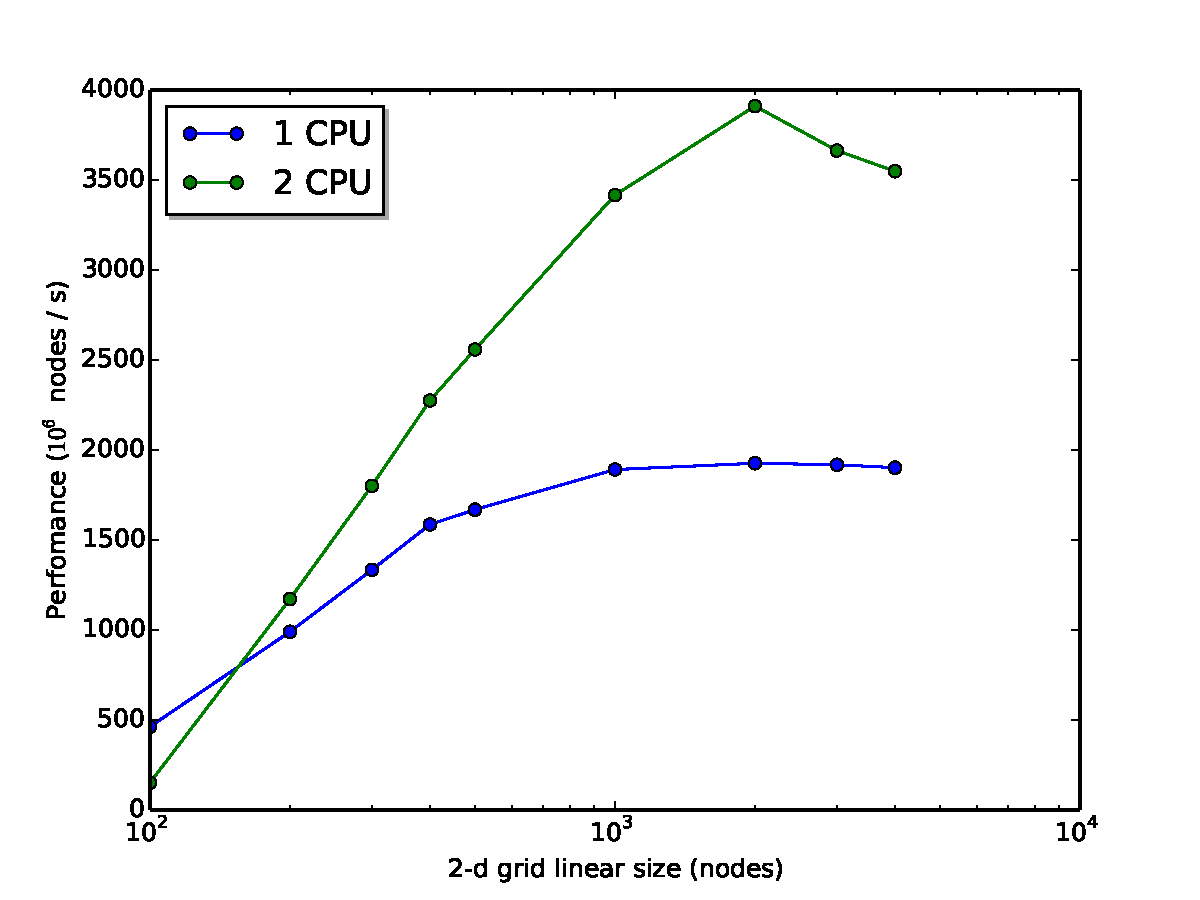
\includegraphics[width=0.65\linewidth]{CPU_1dev_2dev.pdf}}
	\caption{Работа одного и двух CPU}
	\label{ris:cpu_1_2}
\end{figure}

\par Как видно из представленного сравнения, производительность расчет с увеличением размера области. Кроме того сочетание двух процессоров при размере стороны квадрата в 4000 элементов увеличивает производительность на 86\%. Подобное увеличение стало возможным благодаря специальному алгоритму расчетов, который был представлен ранее. За счет "<маскировки"> пересылок расчетами центральных элементов вычислительные мощности практически никогда не простаивают.

\par Следующий график сравнивает производительность центрального процессора и видеокарты (см. Рис.~\ref{ris:cpu_1_gpu_1}).
\begin{figure}[h]
	\center{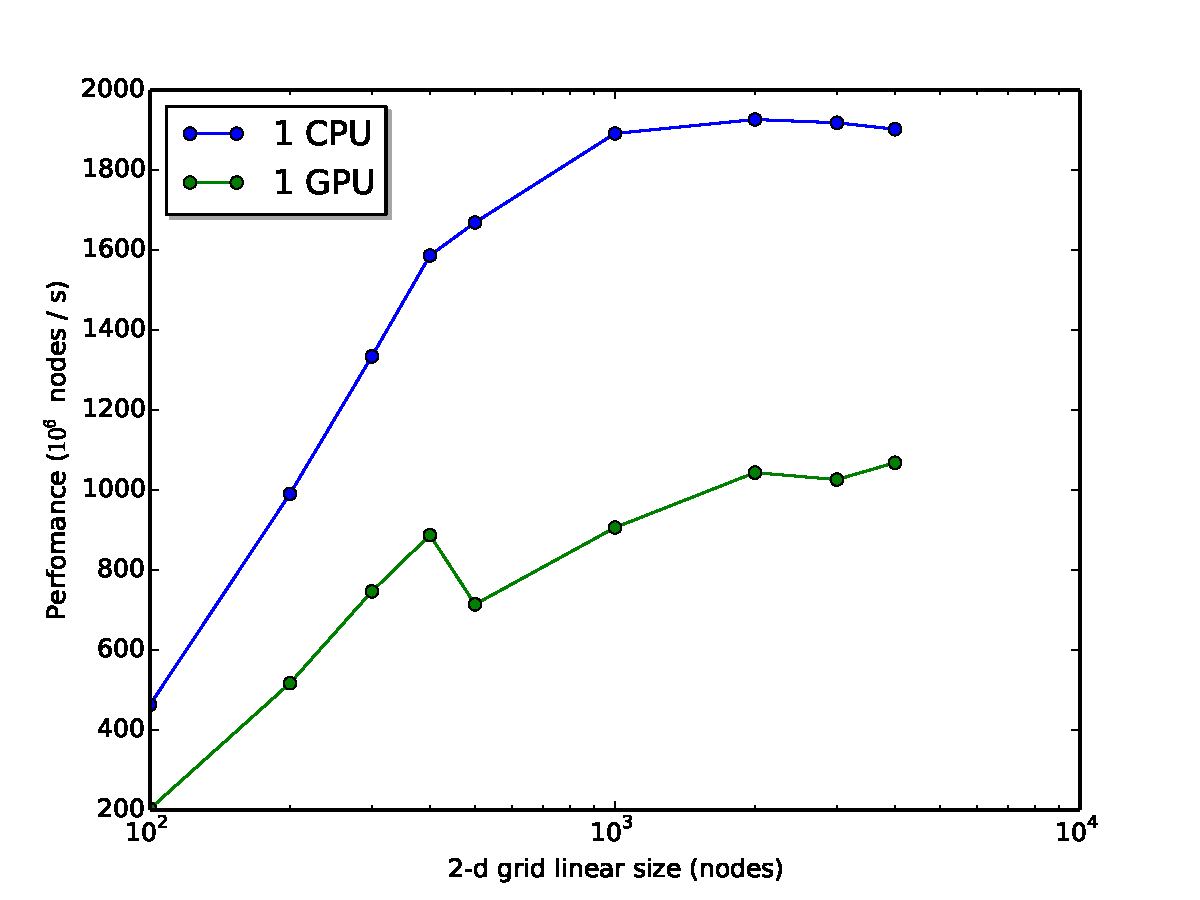
\includegraphics[width=0.65\linewidth]{CPU_GPU_1dev.pdf}}
	\caption{Работа CPU и GPU}
	\label{ris:cpu_1_gpu_1}
\end{figure}

\par При анализе данного графика были получены неожиданные результаты. Традиционно считается, что видеокарты эффективнее осуществляют расчеты, но в данном случае процессор оказался значительно быстрее. Подобный эффект возникает, во-первых, из-за использования арифметики двойной точности, что отрицательно сказывается на скорости обработки данных видеокартой, а, во-вторых, особенностями алгоритма вычисления нового состояния. Вычисления, проводимые в два этапа (центральные и граничные элементы), приводят к значительному понижению производительности видеокарт. Если же новое состояние вычислять одноэтапно, то во время пересылки данных между узлами кластера оба типа вычислительных устройств (центральный процессор и видеокарта) будут простаивать, что в конечном итоге отрицательно скажется на производительности программного комплекса в целом. Подобный отрицательный эффект будет на порядок замедлять работу в сравнении с потерями при подобных расчетах на видеокартах.

\par Следующий график сравнивает производительность одной и двух видеокарт в пределах одного узла (см. Рис.~\ref{ris:gpu_1_2}). Здесь результаты были вполне ожидаемы. Две видеокарты работают в два раза быстрее, чем одна.
\begin{figure}[h]
	\center{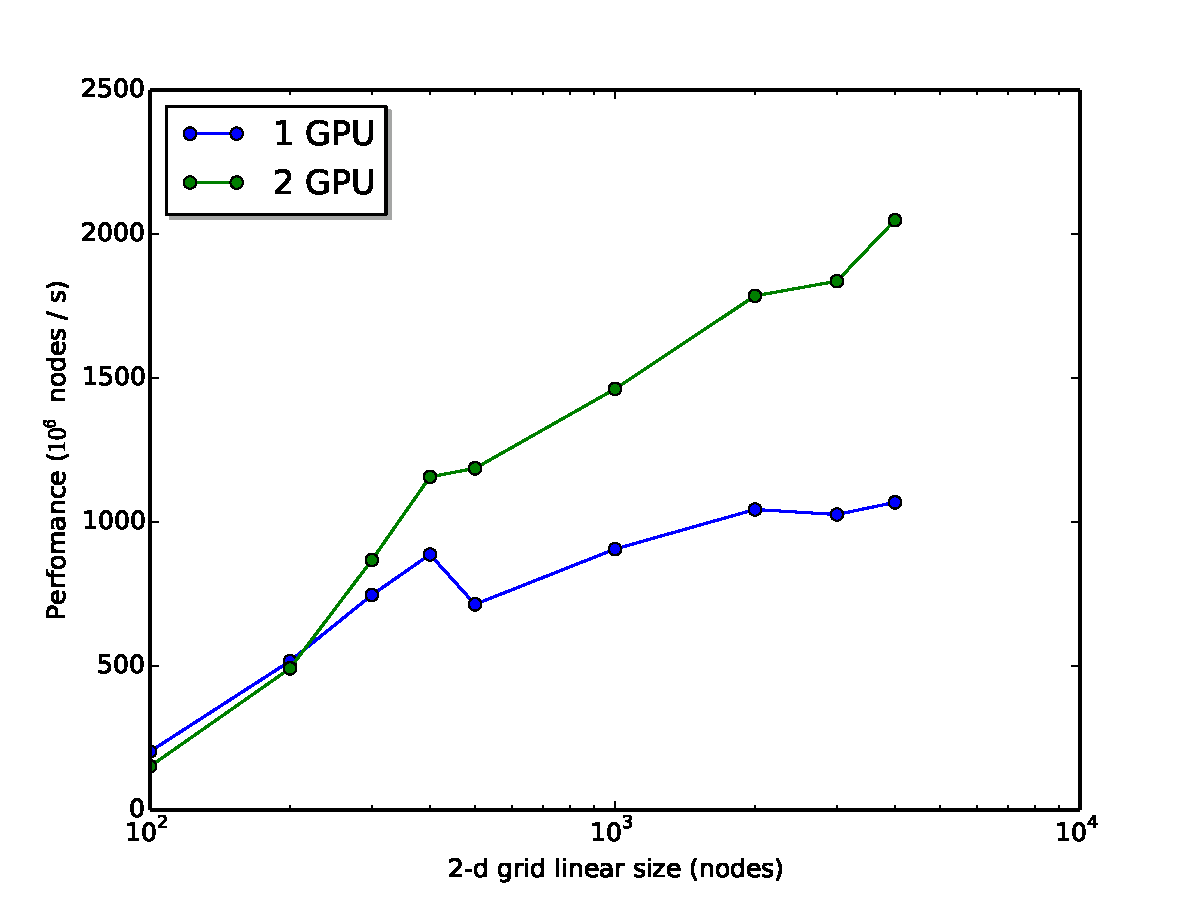
\includegraphics[width=0.65\linewidth]{GPU_1dev_2dev.pdf}}
	\caption{Работа одного и двух GPU}
	\label{ris:gpu_1_2}
\end{figure}

\par Последний график иллюстрирует производительность двух центральных процессоров, расположенных на разных узлах кластера, и двух видеокарт в пределах одного узла (см. Рис.~\ref{ris:cpu_2_gpu_2}).
\begin{figure}[h]
	\center{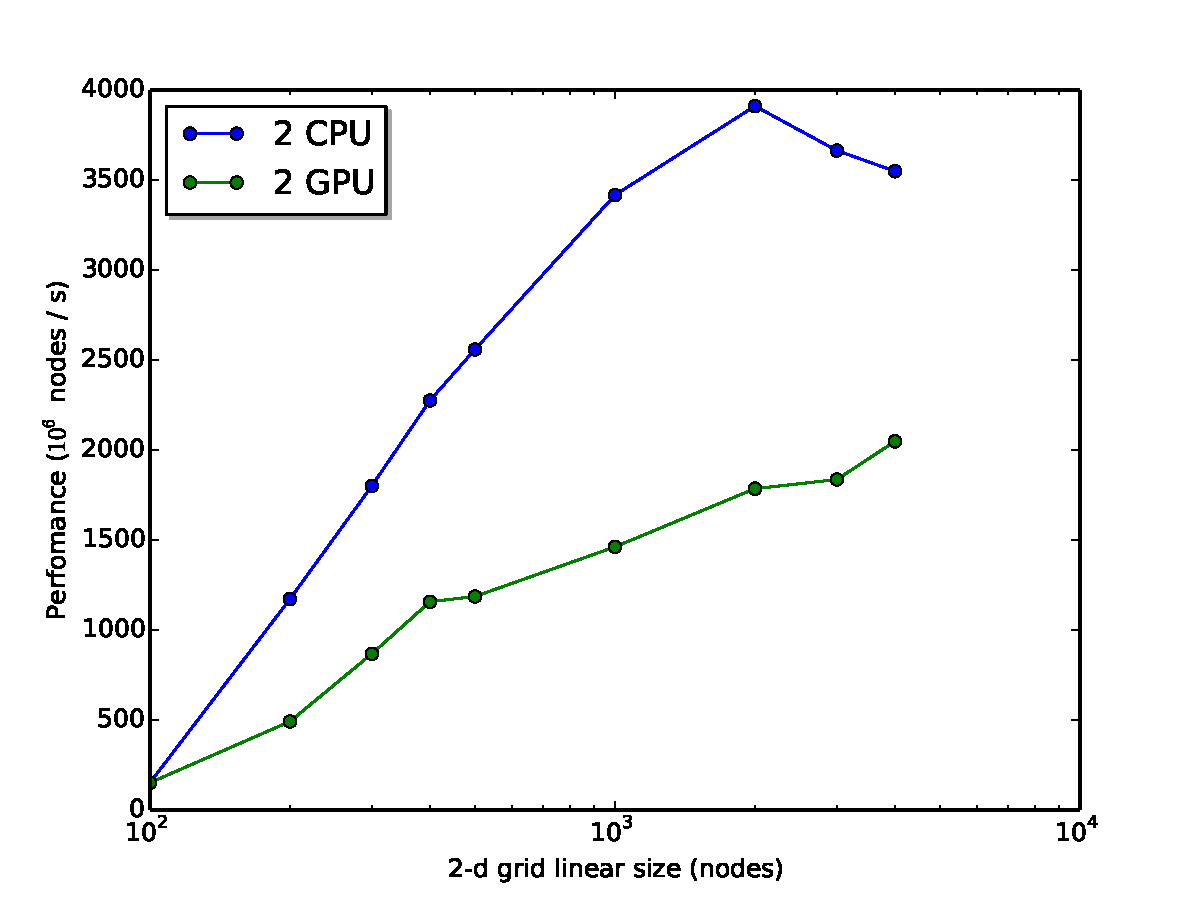
\includegraphics[width=0.65\linewidth]{CPU_GPU_2dev.pdf}}
	\caption{Работа 2xCPU и 2xGPU}
	\label{ris:cpu_2_gpu_2}
\end{figure}

\par На рисунке ~\ref{ris:hist} представлено сравнение производительности различных комбинаций устройств.
\begin{figure}[h]
	\center{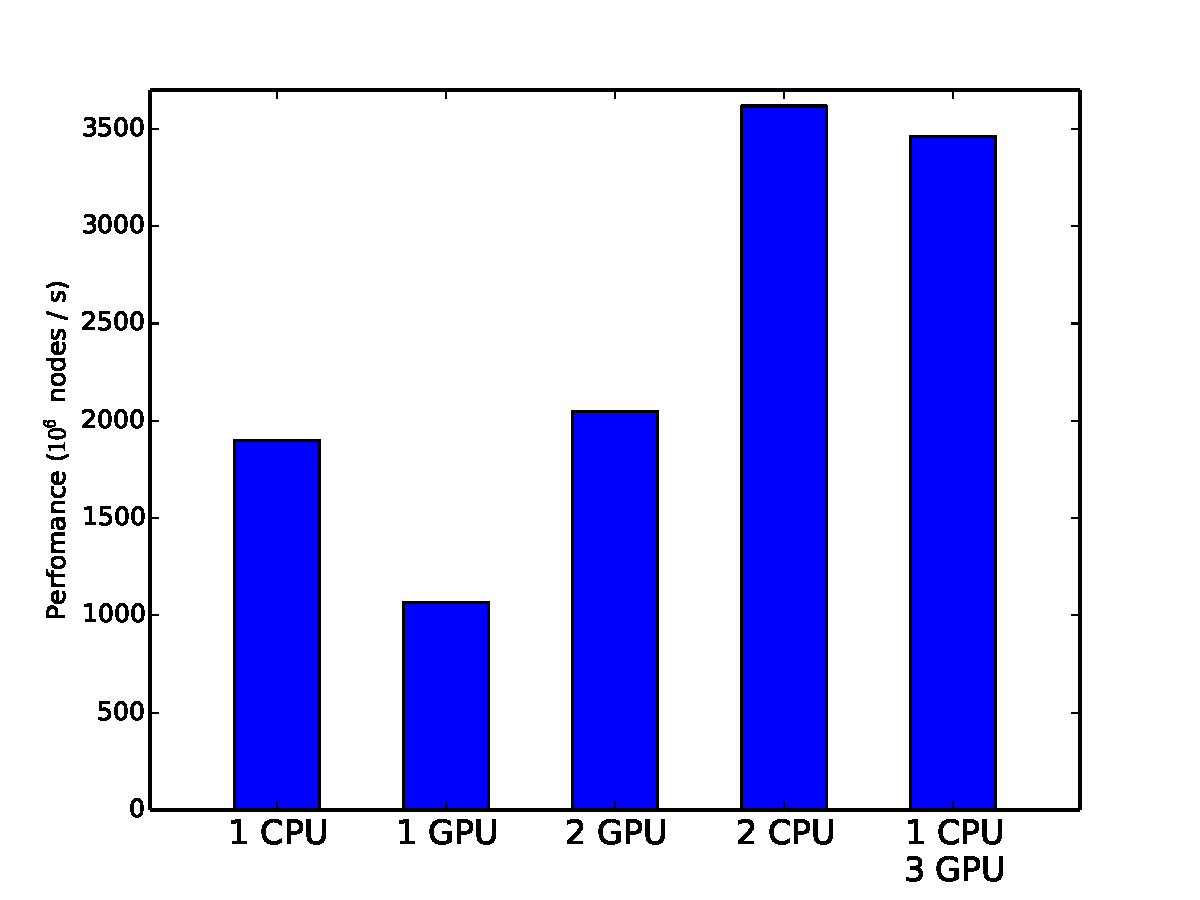
\includegraphics[width=0.65\linewidth]{hist.pdf}}
	\caption{Различные комбинации устройств}
	\label{ris:hist}
\end{figure}

\par Наиболее эффективно производится обработка данных с использованием двух процессоров. Чуть медленнее работает комбинация из одного процессора и трех видеокарт. Почти с одинаковой скоростью осуществляют вычисления процессор и две видеокарты. Важно отметить, что процессор почти в два раза быстрее графического ускорителя. Наименее эффективное устройство -- одна видеокарта.

\par Вывод очевиден: основную нагрузку при расчетах следует отдавать центральному процессору, видеокарту нужно использовать для обработки блоков меньшего размера.



%Заключение
\section*{Заключение}
\addcontentsline{toc}{section}{Заключение}

\par В настоящее время задача автоматизации моделирования задач "<реакция-диффузия"> предъявляет к разработчику новые требования, которые связаны как с повышением уровня абстракции, так и с увеличением производительности вычислений.

\par Для решения указанной задачи автоматизации был разработан программный комплекс, представленный в данной работе. Автором работы реализована часть приложения, отвечающая за повышения производительности.

\par В процессе создания программного комплекса автором работы на первом этапе были изучены теоретические основы численного решения дифференциальных уравнений или систем уравнений с применением методов Эйлера, Рунге-Кутты и Дормана-Принса. На втором этапе были сформулированы основные требования к программному комплексу, в том числе в части описания области моделирования и использования гибридных вычислительных кластеров. С учетом выдвинутых требований автором работы в качестве языка программирования был выбран язык C++ как наиболее соответствующий поставленным задачам.

\par На следующем этапе проекта было необходимо разработать архитектуру описываемой части программного комплекса. Автором работы был предложен следующий вариант архитектуры. Для реализации численного метода используется класс Solver и его наследники. Для отображения в приложении составляющих частей области задачи применяются наследники класса Block. Для управления работой по передаче данных -- класс Interconnect. Общее руководство вычислениями осуществляется с помощью класса Domain. В настоящей работе автором представлено подробное описание используемых классов, а также примерная схема вычислений с использованием центрального процессора и видеокарт.

\par Для решения поставленной перед автором задачи, связанной с увеличением производительности, были использованы так называемые распределенные вычисления, проводимые в две стадии. На первой стадии применяются идеи крупнозернистого параллелизма, а именно разбиение области задачи на блоки и распределение их по вычислительным устройствам. Вторая стадия предполагает реализацию параллельности вычислений с помощью библиотеки OpenMP и языка CUDA в зависимости от типа устройств, на которых эти вычисления осуществляются. Данный подход носит название мелкозернистого параллелизма. Отдельное внимание в работе уделено передаче информации между узлами вычислительного кластера, которая реализована с помощью библиотеки MPI.

\par На последнем этапе проекта автором работы проведено тестирование программного комплекса в части повышения производительности при увеличении количества имеющихся вычислительных устройств. В качестве тестовой задачи было использовано уравнение теплопроводности, распределенное в прямоугольной области. Тестирование показало, что увеличение количества вычислительных устройств положительно сказывается на производительности. При этом получены неожиданные результаты, связанные с тем, что центральный процессор показал лучшую производительность по сравнению с видеокартой. Автором работы было сделано предположение, что описанный эффект связан с особенностями алгоритма вычислений.

\par Поставленная задача реализована автором работы в полном объеме. Тем не менее есть возможность улучшения программного комплекса, в частности, за счет реализации решения задач с запаздыванием.






%Список литературы
\begin{thebibliography}{99}
\addcontentsline{toc}{section}{Список литературы}

\bibitem{pr_first}
\textit{Глызин С.\,Д., Шокин П.\,Л. } 
{Диффузионный хаос в задаче «реакция–диффузия» c гантелеобразной областью определения пространственной переменной. 
М.: Модел. и анализ информ. систем, 2013. -- 43--57 с. }

\bibitem{pr_second}
\textit{Глызин С.\,Д. } 
{Размерностные характеристики диффузионного хаоса. 
М.: Модел. и анализ информ. систем, 2013. -- 30--51 с. }

\bibitem{pr_third}
\textit{Антонов А.\,С. } 
{Параллельное программирование с использованием OpenMP. 
М.: Изд-во МГУ, 2009. -- 77 с. } 

\bibitem{pr_forth}
\textit{Сандерс Дж., Кэндрот Э. } 
{Технология CUDA в примерах. Введение в программирование графических процессоров. 
М.: ДМК Пресс, 2013. -- 232 с. } 

\end{thebibliography}




\newpage

\begin{flushright}
Приложение А
\end{flushright}
\addcontentsline{toc}{section}{Приложение А}

%\begin{center}
%\textbf{Диаграмма классов классификации}
%\end{center}
%
%\center{\includegraphics[width=1\linewidth]{classification_scheme_of_classes_trim.png}}

\begin{lstlisting}
svm_boost::svm_boost(const keypoint_list_lvset& kpl) {
  ...

  int len = kpl.len();
  _dim = kpl.dim();

  svm_node **x = new svm_node*[len]; // List of points in training set
  for (int i = 0; i < len; ++i) {
    x[i] = new svm_node[_dim + 1]; // Point (with index i) of training set
  }
  double *y = new double[len]; // Classes of training set(integers for classification, starting with one)

  for (int i = 0; i < len; i++) {
    y[i] = kpl.loading(i);
    for (int j = 0; j < _dim; j++) {
      x[i][j].value = kpl.get(i, j);
      x[i][j].index = j + 1;
    }
    x[i][_dim].index = -1;
  }

  // Move training set to svm_problem
  _svm_problem = new svm_problem;
  _svm_problem->l = len;
  _svm_problem->y = y;
  _svm_problem->x = x;
	
  ...
}
\end{lstlisting}

\end{document}


















